\documentclass[12pt]{article}

\usepackage[margin=1in]{geometry}
\usepackage[T1]{fontenc}
\usepackage{lmodern}
\usepackage{microtype}
\usepackage{amsmath,amssymb,mathtools}
\usepackage{booktabs}
\usepackage{enumitem}
\usepackage{setspace}
\usepackage{xcolor}
\usepackage{tikz}
\usepackage{hyperref}
\usepackage{xurl}

\hypersetup{
  colorlinks=true,
  linkcolor=black,
  citecolor=black,
  urlcolor=blue,
  pdftitle={Three Powers of Radius: Compactness, Acceleration Scale, and Orbital Rate},
  pdfauthor={Light-Meter Physics},
  pdfsubject={Dimensionless compactness, inverse-time scale, and circular-orbit rate},
  pdfkeywords={compactness, Schwarzschild clock rate, Newtonian gravity, circular orbit, Schuler period}
}

\onehalfspacing
\widowpenalty=10000
\clubpenalty=10000
\definecolor{ink}{HTML}{172E3D}
\definecolor{teal}{HTML}{126D77}
\definecolor{rust}{HTML}{B1533E}
\definecolor{violet}{HTML}{796493}

\title{Three Powers of Radius:\\
Compactness, Acceleration Scale, and Orbital Rate}
\author{Light-Meter Physics}
\date{}

\begin{document}

\maketitle

\begin{abstract}
For a fixed spherical source mass $M$, three familiar quantities vary with radius as $r^{-1}$, $r^{-2}$, and $r^{-3}$. This manuscript derives them from the gravitational time $\tau_g=GM/c^3$ and the radius-time $t_r=r/c$. Their successive forms are the dimensionless compactness $x=\tau_g/t_r$, the inverse-time scale $f_g=\tau_g/t_r^2=g_N/c$, and the squared circular-orbit rate $\Omega_K^2=\tau_g/t_r^3=GM/r^3$. The first quantity sets the leading weak-field excess of the inverse rate of a clock held at fixed radius in Schwarzschild spacetime. The second is an acceleration scale expressed in inverse-time units, not an oscillator frequency. The third follows both from differentiating the Newtonian inverse-square field and from the circular-orbit equation. Earth and solar examples illustrate the scaling and its limits. The manuscript distinguishes exact definitions and derivatives from weak-field expansions and model-dependent physical interpretations; it introduces no new law of gravity.
\end{abstract}

\noindent\textbf{Keywords:} compactness, Schwarzschild clock rate, inverse-time scale, circular orbit, Schuler period

\section{Introduction}
\label{sec:introduction}

The gravitational influence of a fixed source becomes weaker with distance, but different questions involve different powers of that distance. A dimensionless measure of compactness scales as $1/r$. The Newtonian field magnitude scales as $1/r^2$. A circular-orbit rate squared and the radial derivative of the Newtonian field magnitude scale as $1/r^3$. These are related quantities, not three independent constants.

The derivation begins with only a source mass $M$, an exterior radius $r$, and the constants $G$ and $c$. Rewriting the source mass and radius as times exposes a simple sequence:
\begin{equation}
  \tau_g\equiv\frac{GM}{c^3},
  \qquad
  t_r\equiv\frac{r}{c},
  \qquad
  x\equiv\frac{\tau_g}{t_r},
  \qquad
  f_g\equiv-\frac{dx}{dt_r}.
  \label{eq:sequence-definitions}
\end{equation}
For fixed $M$, these definitions lead to $x=GM/(rc^2)$ and $f_g=g_N/c$. The first is a relativistic compactness parameter; the second is an inverse-time scale associated algebraically with the Newtonian field. In Sec.~\ref{sec:third-rung}, $\Omega_K$ is introduced independently as the angular rate of a Newtonian circular test-particle orbit. Circular force balance gives $\Omega_K^2=GM/r^3$, which also equals $-\tfrac12\,dg_N/dr$ for the inverse-square field.

The discussion keeps those interpretations separate. The clock-rate result comes from the exterior Schwarzschild metric and its weak-field expansion. The field and orbit results are developed in the Newtonian point-source model. A short appendix shows that the same circular-orbit coordinate rate also follows for Schwarzschild circular geodesics when time is normalized at infinity. All numerical examples are idealized comparisons, not measurements of actual surface orbits.

\section{Model, notation, and units}
\label{sec:model}

Let $M$ be the mass parameter of a spherical, nonrotating source, and let $r$ be the areal radius outside that source. In the Schwarzschild calculation, $t$ is the time coordinate normalized to the proper time of a static observer at infinity. The Schwarzschild exterior describes the vacuum region outside a spherical nonrotating body \cite{TongGR}.

The radius-time $t_r=r/c$ is a convenient unit conversion, not the elapsed proper time of an observer and not, in general, the travel time of a light signal from the source to radius $r$. The gravitational time $\tau_g=GM/c^3$ is likewise a scale formed from the source's mass parameter. Their units and derived quantities are:
\begin{center}
\small
\begin{tabular}{@{}lll@{}}
  \toprule
  Symbol & Definition or meaning & SI unit \\
  \midrule
  $\tau_g$ & gravitational time $GM/c^3$ & $\mathrm{s}$ \\
  $t_r$ & radius-time $r/c$ & $\mathrm{s}$ \\
  $x$ & compactness $\tau_g/t_r$ & dimensionless \\
  $g_N$ & Newtonian field magnitude $GM/r^2$ & $\mathrm{m\,s^{-2}}$ \\
  $f_g$ & inverse-time scale $g_N/c$ & $\mathrm{s^{-1}}$ \\
  $\Omega_K$ & Newtonian circular-orbit angular rate & $\mathrm{s^{-1}}$ \\
  \bottomrule
\end{tabular}
\end{center}

Here $f_g$ is a quantity with units of inverse time. Calling it a frequency scale does not mean it counts cycles or describes an oscillator. The angular rate $\Omega_K$ does describe circular motion in the specified orbit model.

\section{First rung: compactness and the static clock rate}
\label{sec:compactness}

From the definitions in Eq.~\eqref{eq:sequence-definitions},
\begin{equation}
  x=\frac{\tau_g}{t_r}
   =\frac{GM/c^3}{r/c}
   =\frac{GM}{rc^2}.
  \label{eq:compactness}
\end{equation}
This is dimensionless and decreases inversely with radius at fixed mass. It is commonly called the compactness parameter for this exterior field.

For a static clock at fixed $r$ in the vacuum exterior and outside the Schwarzschild radius, $r>2GM/c^2$, the metric gives
\begin{equation}
  ds^2=-\left(1-\frac{2GM}{rc^2}\right)c^2dt^2
  \quad\Longrightarrow\quad
  \alpha\equiv\frac{d\tau}{dt}=\sqrt{1-2x}.
  \label{eq:static-lapse}
\end{equation}
Use the project notation for the inverse clock-rate ratio,
\begin{equation}
  \delta\tau_{\rm static}
  \equiv\frac{dt}{d\tau}
  =\frac{1}{\alpha}
  =\frac{1}{\sqrt{1-2x}}.
  \label{eq:static-inverse-rate}
\end{equation}
The quantity $\delta\tau_{\rm static}$ is dimensionless; it is not an elapsed proper-time interval. Its excess over unity is exactly
\begin{equation}
  \epsilon_{\rm grav}
  \equiv\delta\tau_{\rm static}-1
  =(1-2x)^{-1/2}-1
  =x+\frac{3}{2}x^2+O(x^3).
  \label{eq:clock-expansion}
\end{equation}
Thus $x$ is the leading, first-order inverse-rate excess only in the weak field, $x\ll1$. The exact relation in Eq.~\eqref{eq:static-inverse-rate} is for a clock held static outside the source. A moving clock has an additional kinematic contribution to $dt/d\tau$ and is not described by that static expression alone.

\section{Second rung: the inverse-time scale}
\label{sec:inverse-time}

At fixed $M$, differentiate compactness with respect to the radius-time. Since $t_r=r/c$, the operation $d/dt_r$ here is the derivative $c\,d/dr$ along the family of radii; it is not a derivative with respect to a clock's elapsed time:
\begin{align}
  f_g
  &\equiv-\frac{dx}{dt_r}
   =-c\frac{d}{dr}\left(\frac{GM}{rc^2}\right) \\
  &=\frac{GM}{cr^2}
   =\frac{g_N}{c}
   =\frac{\tau_g}{t_r^2},
  \qquad g_N\equiv\frac{GM}{r^2}.
  \label{eq:inverse-time-scale}
\end{align}
The sign is chosen so that $f_g$ is positive as the inward field magnitude decreases outward. Its units are $\mathrm{s^{-1}}$, because acceleration divided by speed has units of inverse time.

Equation~\eqref{eq:inverse-time-scale} is an algebraic connection between compactness's radial slope and the Newtonian field scale. It does not make $f_g$ a measured cycle frequency. In an inertial Newtonian frame, a test body accelerates inward under this field; an ideal accelerometer carried by the freely falling body reads zero.

\section{Third rung: the field gradient and orbital rate}
\label{sec:third-rung}

For a point source in Newtonian gravity, the inward acceleration has magnitude $g_N=GM/r^2$. For a circular test-particle orbit, define $\Omega_K$ as the magnitude of the orbital angular rate. Circular force balance gives
\begin{equation}
  r\Omega_K^2=g_N=\frac{GM}{r^2}
  \quad\Longrightarrow\quad
  \Omega_K^2=\frac{g_N}{r}=\frac{GM}{r^3}=\frac{\tau_g}{t_r^3}.
  \label{eq:newtonian-orbit-rate}
\end{equation}
Independently, differentiating the inverse-square field magnitude gives
\begin{equation}
  \frac{dg_N}{dr}=-\frac{2GM}{r^3},
  \qquad
  -\frac{1}{2}\frac{dg_N}{dr}
  =\frac{GM}{r^3}
  =\Omega_K^2.
  \label{eq:third-rung-gradient}
\end{equation}
The factor of $1/2$ compensates for the factor of $2$ from differentiating an inverse-square field. Newtonian inverse-square gravity and the circular test-particle model are the assumptions in this derivation \cite{NASAFlight}.

For two initially comoving test probes with a small outward radial separation $\xi_r$, the signed inward acceleration is $a_r=-g_N$. To first order in $\xi_r$,
\begin{equation}
  \Delta a_r\simeq\frac{da_r}{dr}\,\xi_r
  =\frac{2GM}{r^3}\,\xi_r
  =2\Omega_K^2\xi_r.
  \label{eq:radial-tide}
\end{equation}
The outer probe accelerates inward less strongly, so the separation begins to grow. This Newtonian relative-acceleration example previews the tidal interpretation developed later; no curvature invariant is needed here.

Following the series notation, let $\tau_S$ denote the time to sweep one radian and $T_S$ the full orbital period:
\begin{equation}
  \tau_S\equiv\frac{1}{\Omega_K},
  \qquad
  T_S\equiv2\pi\tau_S
      =\frac{2\pi}{\Omega_K}
      =2\pi\sqrt{\frac{t_r^3}{\tau_g}}.
  \label{eq:period}
\end{equation}

\subsection{An idealized Schuler comparison}

For a spherical Earth of radius $R$ with $g_N=GM/R^2$, the ideal Schuler oscillator has angular rate $\omega_S$ satisfying $\omega_S^2=g_N/R=GM/R^3$. Its angular scale therefore matches $\Omega_K$ for the limiting circular orbit just above the surface of an ideal airless sphere. The oscillator and orbit remain distinct physical systems. With the rounded Earth inputs in Table~\ref{tab:scale-examples}, the model gives $T_S=84.3473\,\mathrm{min}$; the cited navigation paper quotes the conventional rounded Schuler period $T_{\rm Sch}=84.4\,\mathrm{min}$ \cite{OliverGower}.

\section{One chain, three radius powers}
\label{sec:radius-powers}

The complete chain, with its meanings kept distinct, is
\begin{equation}
  \boxed{
  x=\frac{\tau_g}{t_r}=\frac{GM}{rc^2},
  \qquad
  f_g=-\frac{dx}{dt_r}=\frac{\tau_g}{t_r^2}=\frac{g_N}{c},
  \qquad
  \Omega_K^2=\frac{\tau_g}{t_r^3}=\frac{GM}{r^3}
  =-\frac12\frac{dg_N}{dr}.}
  \label{eq:three-rungs}
\end{equation}
For fixed mass, doubling the radius halves $x$, quarters $f_g$, and reduces $\Omega_K^2$ by a factor of eight. Consequently, the one-radian time grows by $2^{3/2}$ and the full period does as well.

At fixed $M$, $d/dt_r=c\,d/dr$ acts along the family of radii. Since $f_g=-dx/dt_r$, the third rung can also be written as the next derivative in the chain:
\begin{equation}
  \Omega_K^2
  =-\frac12\frac{df_g}{dt_r}
  =\frac12\frac{d^2x}{dt_r^2}.
  \label{eq:derivative-ladder}
\end{equation}
The orbital derivation above identifies this derivative scale independently as the circular-orbit rate squared.

\begin{figure}[ht]
  \centering
  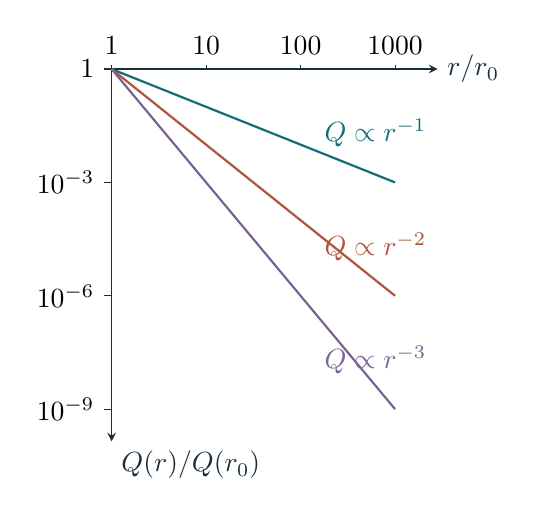
\begin{tikzpicture}[x=1.2cm,y=0.48cm,>=stealth]
    \draw[->,ink] (0,0)--(3.45,0)
      node[right] {$r/r_0$};
    \draw[->,ink] (0,0)--(0,-9.85)
      node[below right] {$Q(r)/Q(r_0)$};
    \foreach \x/\label in {0/1,1/10,2/100,3/1000}{
      \draw[ink] (\x,0)--(\x,0.12);
      \node[above] at (\x,0.12) {$\label$};
    }
    \foreach \y/\label in {0/1,-3/10^{-3},-6/10^{-6},-9/10^{-9}}{
      \draw[ink] (0,\y)--(-0.08,\y);
      \node[left] at (-0.08,\y) {$\label$};
    }
    \draw[thick,teal] (0,0)--(3,-3);
    \draw[thick,rust] (0,0)--(3,-6);
    \draw[thick,violet] (0,0)--(3,-9);
    \node[anchor=west,teal] at (2.15,-1.7) {$Q\propto r^{-1}$};
    \node[anchor=west,rust] at (2.15,-4.7) {$Q\propto r^{-2}$};
    \node[anchor=west,violet] at (2.15,-7.7) {$Q\propto r^{-3}$};
  \end{tikzpicture}
  \caption{Normalized radius dependence of the three rungs. Each quantity is divided by its value at a reference radius $r_0$, so the plot compares scaling laws rather than dimensional magnitudes. Both axes use logarithmic scales. The slopes are $-1$, $-2$, and $-3$.}
  \label{fig:radius-powers}
\end{figure}

\section{Worked scale comparison}
\label{sec:examples}

Use the Earth gravitational parameter, the rounded mean radius $R=6{,}371.0\,\mathrm{km}$, the solar gravitational parameter, and the exact astronomical unit as stated inputs \cite{JPLParams,JPLPhysical}. JPL lists the Earth's mean radius as $6{,}371.0084\,\mathrm{km}$; the rounded value is retained as the model input. Treat each source as spherical and each orbit as a Newtonian circular test-particle orbit. The Earth-at-$R$ case is the limiting circular orbit just above the surface of an ideal airless sphere, not a physical orbit through the planet.

\begin{table}[ht]
  \centering
  \small
  \begin{tabular}{@{}lccc@{}}
    \toprule
    Quantity & Earth at $R$ & Earth at $2R$ & Sun at $1\,\mathrm{AU}$ \\
    \midrule
    $t_r$ ($\mathrm{s}$) & $0.0212514$ & $0.0425027$ & $499.005$ \\
    $\tau_g$ ($\mathrm{s}$) & $1.47937\times10^{-11}$ & $1.47937\times10^{-11}$ & $4.92549\times10^{-6}$ \\
    $x$ & $6.96127\times10^{-10}$ & $3.48064\times10^{-10}$ & $9.87063\times10^{-9}$ \\
    $f_g$ ($\mathrm{s^{-1}}$) & $3.27568\times10^{-8}$ & $8.18921\times10^{-9}$ & $1.97806\times10^{-11}$ \\
    $\Omega_K^2$ ($\mathrm{s^{-2}}$) & $1.54140\times10^{-6}$ & $1.92675\times10^{-7}$ & $3.96402\times10^{-14}$ \\
    $\tau_S$ & $13.4243\,\mathrm{min}$ & $37.9696\,\mathrm{min}$ & $58.1324\,\mathrm{d}$ \\
    $T_S$ & $84.3473\,\mathrm{min}$ & $238.570\,\mathrm{min}$ & $365.2569\,\mathrm{d}$ \\
    \bottomrule
  \end{tabular}
  \caption{Illustrative values computed from $\tau_g=GM/c^3$ and $t_r=r/c$. Earth values use $GM_\oplus=3.98600435507\times10^{14}\,\mathrm{m^3\,s^{-2}}$ and the rounded model input $R=6{,}371{,}000\,\mathrm{m}$; the solar example uses $GM_\odot=1.32712440041279419\times10^{20}\,\mathrm{m^3\,s^{-2}}$ and $1\,\mathrm{AU}=149{,}597{,}870{,}700\,\mathrm{m}$. Displayed values are rounded.}
  \label{tab:scale-examples}
\end{table}

At Earth radius $R$, the ideal one-radian time is $\tau_S\simeq13.42$ minutes and the ideal circular period is $T_S\simeq84.35$ minutes. At $2R$, the third rung is one-eighth as large and the period is $2^{3/2}$ times longer. At one astronomical unit, the same Newtonian relation gives $\tau_S\simeq58.13$ days and $T_S\simeq365.26$ days.

\section{Interpretive limits}
\label{sec:limits}

The derivations support a small set of specific statements:
\begin{itemize}[leftmargin=*]
  \item $x=GM/(rc^2)$ is the exact compactness ratio defined here. Its interpretation as a static inverse-clock-rate excess is only first order in the weak field; the exact clock expression applies to a static clock in the exterior Schwarzschild geometry.
  \item $f_g=g_N/c$ is an inverse-time scale constructed from the Newtonian field magnitude. It is not an oscillator frequency or a freely falling observer's accelerometer reading.
  \item $\Omega_K^2=GM/r^3$ follows from the Newtonian circular test-particle equation and from the derivative of the Newtonian inverse-square field. Neither identity by itself supplies a force history or describes a noncircular orbit.
  \item The Schuler comparison is a shared angular scale in an ideal spherical-Earth model, not an assertion that an inertial-navigation system and a satellite follow the same dynamics.
  \item The compactness, field, and orbital-rate quantities have different units and operational meanings. Their common mass-and-radius construction does not make them interchangeable.
  \item Evaluating $x$ at the Schwarzschild radius gives $x=1/2$, but the weak-field expansion fails there and the static-clock expression cannot describe a clock held at the horizon. The numerical table contains no strong-field extrapolation.
\end{itemize}

\section{Conclusion}

The three radius powers follow from two time scales. Their ratios produce the compactness $x=\tau_g/t_r$. Taking its negative derivative with respect to $t_r$ at fixed $M$ gives $f_g=\tau_g/t_r^2=g_N/c$. The inverse-square field's radial slope, and the Newtonian circular-orbit equation, give $\Omega_K^2=\tau_g/t_r^3=GM/r^3$.

The chain is useful because it organizes several standard results in one notation. Its interpretation still depends on context: compactness enters the exact static Schwarzschild clock rate, the first-order clock excess is weak-field only, the inverse-time scale is not a physical oscillator frequency, and the orbital result assumes a specified circular-orbit model. The powers of radius are connected by algebra and calculus; they are not a new gravitational law.

\appendix

\section{Circular coordinate rate in Schwarzschild spacetime}
\label{app:schwarzschild-orbit}

The coordinate angular rate of a circular Schwarzschild geodesic follows directly. In the equatorial plane, write
\begin{equation}
  ds^2=-F(r)c^2dt^2+F(r)^{-1}dr^2+r^2d\phi^2,
  \qquad
  F(r)=1-\frac{2GM}{rc^2}.
  \label{eq:schwarzschild-equatorial}
\end{equation}
For a circular geodesic, $r$ is constant. The radial geodesic equation then reduces to
\begin{equation}
  0=\Gamma^r{}_{tt}\left(\frac{dt}{d\tau}\right)^2
    +\Gamma^r{}_{\phi\phi}\left(\frac{d\phi}{d\tau}\right)^2,
  \qquad
  \Gamma^r{}_{tt}=F\frac{GM}{r^2},
  \qquad
  \Gamma^r{}_{\phi\phi}=-Fr.
  \label{eq:circular-radial-geodesic}
\end{equation}
Canceling $F$ and forming the coordinate rate with respect to Schwarzschild time gives
\begin{equation}
  \Omega\equiv\frac{d\phi}{dt},
  \qquad
  \Omega^2=\frac{GM}{r^3}.
  \label{eq:schwarzschild-coordinate-rate}
\end{equation}
Using $d\tau^2=-ds^2/c^2$ for the massive circular orbit and substituting $r^2\Omega^2=GM/r$ into the line element gives
\begin{equation}
  \left(\frac{d\tau}{dt}\right)^2
  =F-\frac{r^2\Omega^2}{c^2}
  =1-\frac{3GM}{rc^2}>0,
  \qquad
  r>\frac{3GM}{c^2}.
  \label{eq:circular-timelike-condition}
\end{equation}
Thus a circular massive geodesic in the vacuum exterior requires $r>3GM/c^2$. The coordinate-rate relation is exact for these circular geodesics, with $t$ normalized at infinity. It does not mean that $r$ is a proper radial distance or that the Newtonian interpretation of every quantity remains valid in the strong field. See the Schwarzschild geodesic treatment in Ref.~\cite{TongGR}.

\section{Numerical and dimensional checks}
\label{app:numerical-checks}

Using $c=299{,}792{,}458\,\mathrm{m\,s^{-1}}$, the source parameters and radii stated in Table~\ref{tab:scale-examples} give
\begin{align}
  \frac{\tau_g}{t_r}
  &=\frac{GM}{rc^2},\\
  \frac{\tau_g}{t_r^2}
  &=\frac{GM}{cr^2}
    =\frac{g_N}{c},\\
  \frac{\tau_g}{t_r^3}
  &=\frac{GM}{r^3}
    =\Omega_K^2.
  \label{eq:dimension-checks}
\end{align}
Their units are respectively dimensionless, $\mathrm{s^{-1}}$, and $\mathrm{s^{-2}}$. For example, at twice the radius,
\begin{equation}
  x(2r)=\frac{x(r)}{2},
  \qquad
  f_g(2r)=\frac{f_g(r)}{4},
  \qquad
  \Omega_K^2(2r)=\frac{\Omega_K^2(r)}{8}.
  \label{eq:doubling-check}
\end{equation}

\begin{thebibliography}{9}
\small
\setstretch{1.0}
\raggedright
\urlstyle{same}

\bibitem{TongGR}
D. Tong,
\emph{General Relativity},
lecture notes, University of Cambridge, Chapters 1 and 6,
available at \href{https://www.damtp.cam.ac.uk/user/tong/gr/grhtml/}{damtp.cam.ac.uk/user/tong/gr/grhtml/}.

\bibitem{NASAFlight}
NASA,
\emph{Basics of Space Flight},
Chapter 3, ``Gravity \& Mechanics,''
available at \href{https://science.nasa.gov/learn/basics-of-space-flight/chapter3-3/}{science.nasa.gov/learn/basics-of-space-flight/chapter3-3/}.

\bibitem{OliverGower}
B. M. Oliver and J. F. R. Gower,
``Use of an inertial navigation system for accurate track recovery and coastal oceanographic measurements,''
Sec.~3, Eq.~(1) (1977), NASA Technical Reports Server, record 19780006643,
available at \href{https://ntrs.nasa.gov/citations/19780006643}{ntrs.nasa.gov/citations/19780006643}.

\bibitem{JPLParams}
NASA Jet Propulsion Laboratory,
Solar System Dynamics, ``Astrodynamic Parameters,''
available at \href{https://ssd.jpl.nasa.gov/astro_par.html}{JPL Astrodynamic Parameters}.

\bibitem{JPLPhysical}
NASA Jet Propulsion Laboratory,
Solar System Dynamics, ``Planetary Physical Parameters,''
available at \href{https://ssd.jpl.nasa.gov/planets/phys_par.html}{JPL Planetary Physical Parameters}.

\end{thebibliography}

\end{document}